\documentclass{standalone}

\usepackage[utf8]{inputenc}
\usepackage{tikz,fp,siunitx}
\usetikzlibrary{decorations.pathreplacing}

\begin{document}
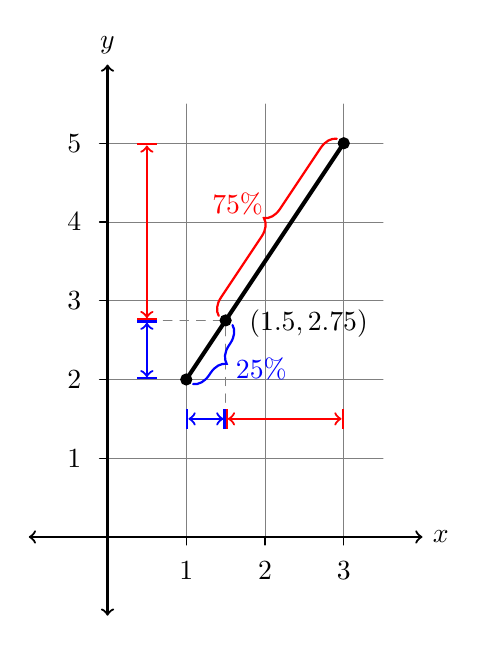
\begin{tikzpicture}[scale=1,cap=round]

   % Grid
   \draw[style=help lines,step=1cm] (0,0) grid (3.5, 5.5);
   
   % Axis line
   \draw[<->,thick] (-1,0) -- (4,0) node[right] {$x$};
   \draw[<->,thick] (0,-1) -- (0, 6) node[above] {$y$};
   
   % Axis strokes
   \foreach \x in {1,2,3}
       \draw[line width=0.5pt] (\x,-0.1) -- (\x, 0) node[yshift=-12pt] {\x};
   \foreach \y in {1,2,...,5}
       \draw[line width=0.5pt] (-0.1,\y) -- (0, \y) node[xshift=-12pt] {\y};

	
	\draw[dashed,gray] (0.5, 2.75) -- (1.5, 2.75);
	\draw[dashed,gray] (0.5, 2.75) -- (1.5, 2.75);

	\draw[dashed,gray] (1.5, 1.5) -- (1.5, 2.75);

 	\draw[|<->|,thick,blue] (0.5, 2) -- (0.5, 2.75);
 	\draw[|<->|,thick,red]  (0.5, 2.75) -- (0.5, 5);
	
 	\draw[|<->|,thick,blue] (1, 1.5) -- (1.5, 1.5);
 	\draw[|<->|,thick,red]  (1.5, 1.5) -- (3, 1.5);


   \draw[line width=1.5] (1,2) -- (3,5);
   \draw plot [mark=*, mark size=2] coordinates{(1,2)};
   \draw plot [mark=*, mark size=2] coordinates{(3,5)};

   \draw plot [mark=*, mark size=2] coordinates{(1.5,2.75)}
         node[xshift=30pt, yshift=-1pt, transparency group=knockout] 
             {$(1.5, 2.75)$};

   \draw[decorate, thick, red,
         decoration={brace, amplitude=6pt, raise=3pt},
         yshift=0pt]
        (1.5,2.75) -- (3, 5)
        node [midway, xshift=-17pt, yshift=10pt] { $75\%$ };

    \draw[decorate, thick, blue,
          decoration={brace, mirror, amplitude=6pt, raise=3pt},
          yshift=0pt]
         (1,2) -- (1.5, 2.75)
         node [midway,xshift=20pt,yshift=-7pt] { $25\%$ };
 

	
   \newcommand{\lineann}[4][0.5]{%
    \begin{scope}[rotate=#2, blue,inner sep=2pt]
        \draw[dashed, blue!40] (0,0) -- +(0,#1)
            node [coordinate, near end] (a) {};
        \draw[dashed, blue!40] (#3,0) -- +(0,#1)
            node [coordinate, near end] (b) {};
        \draw[|<->|] (a) -- node[fill=white] {#4} (b);
    \end{scope}
   }

\end{tikzpicture}

\end{document}
